\documentclass[12pt,a4paper]{article}
\usepackage[utf8]{inputenc}
\usepackage[english,german]{babel}
\usepackage{amsmath}
\usepackage{amsfonts}
\usepackage{amssymb}

\usepackage{fancyhdr}
\usepackage{lastpage}

\usepackage{lastpage}
\usepackage{enumerate}
\usepackage{graphicx}
\usepackage{setspace}
\usepackage{hyperref}

\usepackage{listings}
\lstset{language=c++}

\title{Currend Trends in Distributed Systems\\\textbf{Apache Storm}\\\large{- Report of the presentation on October 16, 2015 -}}
\date{}
\author{Patrick Zumsteg, Philipp Oldenburg, Simon Wallny}

\begin{document}
\selectlanguage{english}
\maketitle
\section*{Abstract}
Bevor wir mit unserem Bericht beginnen, möchte ich ein paar Worte sagen. Und hier sind sie: Schwachkopf! Schwabbelspeck! Krimskrams! Quiek! Danke sehr!
\tableofcontents
\section{What is Storm?}
\onehalfspacing
Apache Storm is an open source framework used to process streams of data on multiple computing nodes. It is written in Clojure (a dialect of Lisp) and has been in development since September 2011. Taken over by Apache in February 2014, Storm is now developed as a Top-Level-Project.\\

Unlike many already existing multi-node computing frameworks, Storm is specifically created to process data as a stream. Furthermore, the computing job which Storm executes, a so-called Topology, doesn't necessarily have to terminate at some point. Therein lie two of the main differences to the otherwise quite similar and more well-known MapReduce-Job, which essentially processes one big batch of input data. Storm on the other hand never stops accepting input data and keeps applying its predefined operations to the incoming data tuples until its services are no longer needed.\\

A Storm cluster is also very resilient. Failures of single nodes go by virtually unnoticed due to Storm's ability to dynamically redistribute unoccupied tasks and even restart crashed nodes.

\section{Basic Architecture}

To understand the functionality of Apache Storm, it is important to first get a grasp of the underlying principles of a multi-node computing system. The following paragraphs will cover the basic building blocks of Storm and, more importantly, how they all work together.

\subsection{Pre-Topology Level: Nodes and Clusters}

As mentioned earlier, Storm aims to distribute workload among all nodes in the so-called Cluster. In Storm, a node can either take the role of the \textbf{Nimbus}, or it can become a \textbf{worker node} (that is, run a \textbf{Supervisor} process). It is important to note, however, that the node itself is not automatically bound to a specific role: On startup, Storm assigns a daemon to each node, and it is this daemon that separates the Nimbus from the ''common workers''.\\

The Nimbus process is basically the control center of the entire Cluster. It is aware of all the tasks which the Topology runs and assigns these tasks to the nodes running a worker daemon. Additionally, the Nimbus contains the code for every one of said tasks. Whenever it assigns a task to a worker, the worker is provided with the code snippet that it is supposed to execute. Another very important functionality of the Nimbus is load balancing: The Nimbus is constantly provided with feedback concerning the effectiveness of its workers. If a worker is unable to efficiently execute its assigned tasks, for example due to it being run on weaker hardware than other nodes, the Nimbus tries to alleviate pressure on said weak node and assign some tasks to another, less busy worker in order to optimize performance.\\

It is important to note that there is only a single Nimbus in every Cluster. This may of course seem counterintuitive at a first glance: If a Cluster contains hundreds or even thousands of worker nodes, this one control node might easily collapse under the sheer pressure that the task of managing every single worker entails. In reality however, the Nimbus utilizes another type of node which exists outside of the Cluster itself, which greatly reduces the processing power required for the Nimbus. But these so-called \textbf{Zookeepers} deserve a section of their own and will be discussed later.\\\\
\indent While the Nimbus handles these more ''intellectual'' tasks like balancing work load, the \textbf{worker processes}, also called \textbf{Supervisors} are, even if their name suggests otherwise, almost the exact opposite. A Supervisor knows nothing of the world surrounding it. It just receives tasks and the code to run them from the Nimbus and executes these tasks until the Nimbus commands them otherwise.\\

As mentioned earlier, the Nimbus is aware of certain state informations about its Supervisors. In an effort to keep the performance requirements of the Nimbus as low as possible, each Supervisor periodically provides this information to the Zookeeper nodes, where it can easily be accessed by the Nimbus.

\subsection{Zookeeper Nodes}

ZooKeeper is another project by Apache. Much like Storm, Zookeeper is generally run on a cluster of nodes. This is, however, not just unnecessary, but actually hinders performance if used in conjuction with Storm, which is why a Storm-Cluster's Zookeeper system often consists of very few or even a single node (this is due to certain limitations of the Zookeeper architecture - more on that later). The purpose of the Zookeeper Cluster is to provide a hierarchical namespace of data registers which is shared among all Zookeeper server nodes. This allows for very fast and reliable storage and exchange of small data.\\

This hierarchical namespace is in many ways quite similar to a file system as we all know it: There is one root node, and every node in the namespace (These nodes are called \textbf{znodes}, not to be confused with server nodes, which are actual devices/VMs) is a child node of another znode and can itself have child nodes linking to it, and all these nodes are uniquely identified by an absolute path. But there are also some major differences to a standard file system, the most important of which is the fact that \textit{every} znode, regardless of it being a file or directory, may have data associated with it. Furthermore, unlike in a normal file system, all data is stored in memory, which is why Zookeeper is able to provide disproportionately fast access to its data.\\


As mentioned earlier, data is transferred to and from the Zookeeper Cluster via a connection to a Zookeeper server node. In order to log its current status information on the Zookeeper system, a Supervisor needs to establish a TCP connection (which is never closed: It would be unreasonable to open a new connection every time since read- and write-requests tend to come in periodically and at a rather high frequency) to a server node and request permission to write into the Zookeeper's file system. This is where one of the weaknesses of Zookeeper becomes evident: Every write-request is passed to \textit{all} the other server nodes, and they must reach consensus before the client is given permission to write (This is necessary to in order to prevent inconsistencies in the data stored on each server). Read-requests however do not need to go through any of this; they are handled locally by the connected server node.\\

Thus, it becomes evident why Storm is better off using as small a Zookeeper Cluster as possible: All nodes except one periodically send write-requests. Lots of them. And the data provided by the Supervisors is tiny, and therefore easily manageable by a single server node.

\section{Topologies}

Now that we've covered the underlying structure with which Storm works, it is time to clarify how the actual work is done. In Storm, all computational tasks are essentially nodes, this time in a graph which is called a \textbf{Topology}. This concept is fairly simple: A Topology is an unweighted, directed graph consisting of \textbf{Spouts} and \textbf{Bolts}. These nodes are then connected by data streams from one node to the other, as is illustrated in the following figure from the Storm website:\\
\begin{center}
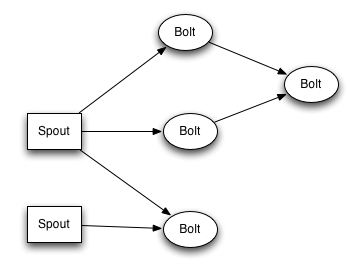
\includegraphics[scale=0.7]{images/topology.png}
\end{center}
Note that every node can potentially be connected to a multitude of Bolts, both through incoming and outgoing streams (Spouts are the exception here. This is due to the different role which the Spouts play in a Topology and will be explained in the following paragraphs)

\subsection{Of Spouts, Bolts and everything in between}

Of course, the Cluster and the Topology aren't just two separate concepts working independently from each other. There is actually a connection between them, and it relies on a type of process mentioned earlier: The \textit{Supervisor}. Although the deeper functionality is much more complex and will be explained later, for now it is important to know that a Supervisor runs a multitude of threads - which are, dependent on their role, called \textit{Spouts} and \textit{Bolts}.\\

As mentioned earlier, Storm was created to process streams of incoming data, and it is therefore reasonable to continue our exploration of the Cluster at the very point where the data enters it as well.

\subsubsection{Spouts}

In Storm, a Spout is the type of node in a Topology which emits one or more streams of data to every node connected to it. This data is usually provided to the Spout by an external service - a good example would be an API from any website which provides data in the form of streams. \\

It is important that every (physical) device on which a \textit{Supervisor} is run actually has access to the original source of data. This is due to the fact that the developer working with Storm has no control over the location where the Spouts and Bolts are actually run; This assignment is done by the Nimbus. It should therefore be assumed that \textit{every} physical device in the Cluster could potentially be selected to have one or more Spouts running on it. In the case of the original data source being a website, this is of course an almost negligible limitation. But if the data originates from a certain process running on a separate machine, the developer has to make the data available to the Spouts by implementing a server.\\

When talking about Spouts, there is an important distinction to make between \textit{reliable} and \textit{unreliable} Spouts. Imagine this like the difference between TCP and UDP: An unreliable Spout simply outputs data without requiring confirmation of any sort; a simple fire-and-forget implementation. A reliable Spout on the other hand provides the tools to check not only if the sent data tuple actually makes it to its recipient, but if the data tuple has completed its entire journey through the Topology. The two methods which a Spout provides to that end are called \textit{ack} and \textit{fail}, which are called whenever a tuple emitted from the Spout successfully completes its journey or fails along the road.

\section{Simons Teil}
\label{sec:Simons Teil}

...kommt hier hin

\section{Apache Storm Setup}
The following 4 steps demonstrate how to setup an Apache Storm Cluster
\subsection{Setup a Zookeeper Cluster}
Depending on how big the Storm Cluster will be the number of Supervisor nodes has to be determined. In cases of small clusters it sufficient to have a Zookeeper cluster with one Zookeeper server only.
The Apache Zookeeper server can be found under the following \href{http://www.eu.apache.org/dist/zookeeper/stable/}{link}. The config file in \path{zookeper/conf/zoo_sample.cfg} should be checked and the following two lines appended, to prevent running out of disk space.
\begin{verbatim}
autopurge.purgeInterval=24
autopurge.snapRetainCount=5  
\end{verbatim}
The server can be started afterwards by running the following script: \path{zookeper/bin/zkServer[.cmd|.sh]}
\subsection{Install dependencies}
Apache Storm has some dependencies for software versions of the Supervisor nodes:
\begin{verbatim}
Java 6
Python 2.6.6
\end{verbatim}
Although some testing has shown that it is also running with newer versions of Java.
\subsection{Nimbus and Supervisor nodes}
The next step includes downloading a distribution of Apache Storm (\href{http://storm.apache.org/downloads.html}{link}) onto the devices which will run the Nimbus server and the Supervisor clients.
To make them run altogether the conif file in \path{apache-storm/conf/storm.yaml} has to changed accordingly. The two attributes, storm.zookeeper.servers and nimbus.host has to be set to IP addresses of the corresponding devices. In case of the Nimbus device they have to be set to "localhost". The attribute storm.local.dir has to be set to some path Storm can place data locally.
\subsection{Setting up Supervisor}
Apache Storm is a fail fast system, which means that it exits if there are any exceptions thrown. To make it run more stable a supervisor program can be used. It basically observes the Nimbus and Supervisor process and restarts them if they break down. A possible software solution would be Supervisor, a process control system, which runs only on UNIX-like operating systems. Download: \href{http://supervisord.org/#}{link}.
To set it up the following lines have to be appended to \path{/etc/supervisord.conf}
\begin{verbatim}
[program:storm-nimbus]
command=/usr/local/storm/bin/storm nimbus
user=storm
autostart=true
autorestart=true
startsecs=10
startretries=999
log_stdout=true
log_stderr=true
logfile=/var/log/storm/nimbus.out
logfile_maxbytes=20MB
logfile_backups=10
\end{verbatim}
The command and logfile path have to be changed accordingly as well as the program name. After setting up the configuration file the supervisor daemon has to be started with: 
\begin{verbatim}
sudo service supervisord start
\end{verbatim}
For troubleshooting:
\begin{verbatim}
sudo supervisorctl status
\end{verbatim}
The sample configuration is this \href{http://www.michael-noll.com/tutorials/running-multi-node-storm-cluster/#install-supervisord}{site}. The page also holds lots of useful information on setting up Apache Storm.
\subsection{Deploying topologies}
After the explanation on how to create a topology in \ref{sec:Simons Teil} the following part describes what to do after the implementation of a cluster.\\
First the coded cluster has to packed with all its packages into a jar file. It is rather important to include only libraries into the jar which are not from Apache Storm. Because including these libraries will end up in a topology which deployable. After successful packing the topology jar can be submitted to the running Storm Cluster via the storm client:
\begin{verbatim}
storm jar path/to/allmycode.jar org.me.MyTopology arg1 arg2 arg3
\end{verbatim}
More information on how to deploy a topology and troubleshooting can be found here: \href{http://storm.apache.org/documentation/Running-topologies-on-a-production-cluster.html}{link}

\end{document}